\documentclass[a4paper]{article}

\usepackage[utf8]{inputenc}
\usepackage[T1]{fontenc}
\usepackage{textcomp}
\usepackage[czech]{babel}
\usepackage{amsmath, amssymb}


% figure support
\usepackage{import}
\usepackage{xifthen}
\pdfminorversion=7
\usepackage{pdfpages}
\usepackage{transparent}
\newcommand{\incfig}[1]{%
    \def\svgwidth{\columnwidth}
    \import{./figures/}{#1.pdf_tex}
}

\pdfsuppresswarningpagegroup=1

\begin{document}
    \begin{section}{Úkol 1}
        Z popisu grafu zjistíme, že existují pouze 3 způsoby, jak rozděilt graf na kružnice, které nebudou totožné, viz obr. \ref{fig:grafy-3}.
    \begin{figure}[htpb]
        \centering
        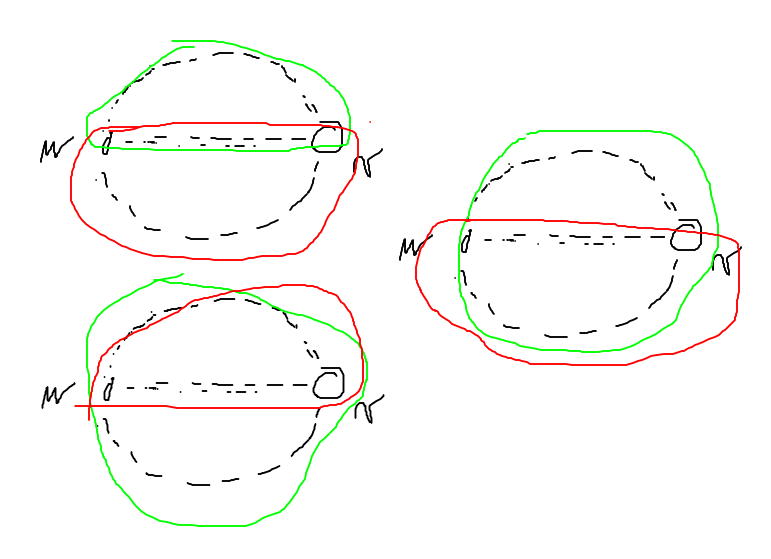
\includegraphics[width=0.8\textwidth]{grafy-3.png}
        \caption{Grafy}
        \label{fig:grafy-3}
    \end{figure}
    Tedy abychom vytvořili konstru, musíme odstranit 2 hrany z dvou různých cyklů na obrázku.
    To lze udělat $m*l + m*k + l*k$ způsoby.
    \end{section}
    \begin{section}{Příklad 2}
        Přidaním hrany nám v grafu vznikne cyklus a zachová se souvislot(strom je maximálně acyklický).
        Každý cyklus má alespoň 3 hrany, proto existují alespoň 2 hrany na nově vzniklém cyklu(3. hrana je ta nově přidaná), které můžeme z nově vzniklého cyklu odebrat a vytvořit tak strom, tedy novou kostru. Tedy právě jsme ukázali, že po přidání hrany budou existovat alespoň 2 jiné hrany, které můžeme odebrat a vytvořit tak novou kostru.
    \end{section}
    \begin{section}{Příklad 3}
        Stačí dokázat pouze případ pro $G \setminus \{u,v\}$, pro $G \setminus \{u\}$ a $G \setminus \{u\}$, poté bude plynout triviálně.
        Každý strom s alespoň 2 vrcholy, má alespoň 2 listy.
        Zároveň pro každý souvislý graf jsme schopni najít kostru.
        Označme si nějakou takou kostru našeho grafu $G$ jako $T$.
        $T$ je z definice souvislá a zárověň pro její kostrukci jenom odebíráme hrany z původního grafu.
        Jelikož je $T$ z definice strom, pak existují dva jeho listy, které můžeme odebrat aniž bychom porušili souvislost(mají stupeň 1). Nově vzniklý graf bez 2 listů $a,b$ označme $S$.
        Nyní celý proces obrátíme a z $S$ vytvoříme původní graf $G \setminus \{a,b\}$.
        Pro každou odebranou hranu $\{u,v\}$ při tvorbě $T$, budeme postupovat následnovně:
        Pokud $\{a,b\} \not \subset\{u,v\}$, danou hranu přidáme do $S$, tedy $E_S \cup \{u,v\}$.
        Jelikož přidáním hran nezměníme souvislost, podařilo se nám odebrat 2 vrcholy z původního grafu a zachovat souvislost. Ještě by se slušelo podotknout, že jelikož má graf $G$ alespoň 3 vrcholu, můžeme 2 odebrat a vznikne nám graf.
    \end{section}
    \begin{section}{Příklad 4}
        Za graf si můžeme vzít cestu délky větší než 3. Protože pokud odebereme z cesty jiný vrchol než krajní,graf se stane nesouvislý. Jelikož množina $M$ obsahuje vždy 3 vrcholy, vždy jsme schopni odebrat jiný vrchol než krajní(krajní vrcholy jsou vždy 2).
        \begin{figure}[htpb]
            \centering
            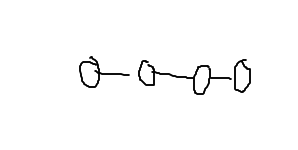
\includegraphics[width=0.8\textwidth]{graf-cesta.png}
            \caption{cesta}
            \label{fig:graf-cesta}
        \end{figure}
        
    \end{section}
\end{document}
